\documentclass[11pt, oneside]{article}   	% use "amsart" instead of "article" for AMSLaTeX format
\usepackage{geometry}                		% See geometry.pdf to learn the layout options. There are lots.
\geometry{letterpaper}                   		% ... or a4paper or a5paper or ... 
%\geometry{landscape}                		% Activate for for rotated page geometry
%\usepackage[parfill]{parskip}    		% Activate to begin paragraphs with an empty line rather than an indent
\usepackage{graphicx}				% Use pdf, png, jpg, or eps� with pdflatex; use eps in DVI mode
								% TeX will automatically convert eps --> pdf in pdflatex		
\usepackage{amssymb}
\usepackage{amsmath}
\usepackage{parskip}
\usepackage{color}
\usepackage{hyperref}

\title{Power series:  convergence}
%\author{The Author}
%\section{}
%\subsection*{}
\date{}							% Activate to display a given date or no date

\graphicspath{{/Users/telliott_admin/Dropbox/Tex/png/}}
% \begin{center} 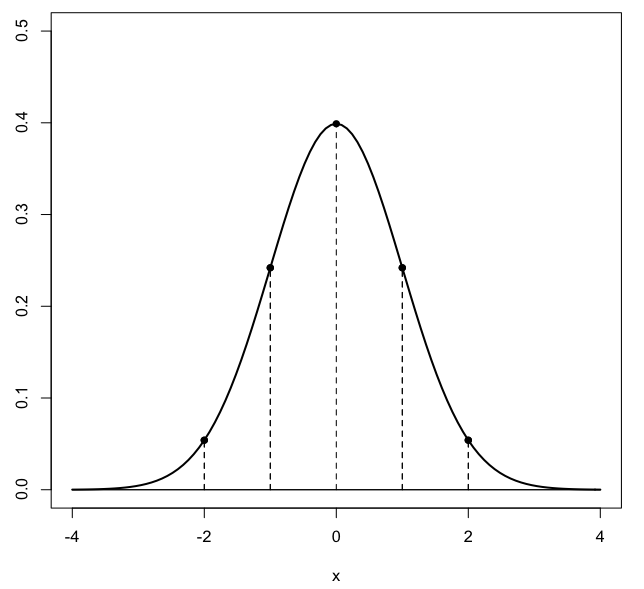
\includegraphics [scale=0.4] {gauss3.png} \end{center}
\begin{document}
\maketitle
\Large
Consider 
\[ \sum_0^{\infty} \frac{x^n}{n!} \]
For real $x$:
\[ e^x = \sum_0^{\infty} \frac{x^n}{n!} \]
This may be used as the definition of the exponential for real $x$.  Now we wish to look at complex $z$.  It turns out to be true that
\[ e^z = \sum_0^{\infty} \frac{z^n}{n!} \]
Following Kharkar, we look at the closely related series
\[ \sum_0^{\infty} (-1)^n \frac{z^n}{n!} \]
We want to determine the radius of convergence of the series.  We use the ratio test to see what happens to successive numbers in the sequence as $n$ gets large.

The ratio test is to look at the ratio of the $n+1$ term to the $n$ term using moduli:
\[ \lim_{n \rightarrow \infty} | \frac{(-1)^{n+1} \ z^{n+1}}{(n+1)!} \ \frac{n!}{(-1)^{n} \ z^{n}} | \]
We can move the absolute value signs to each term, and when we do that the terms with $-1$ go away so
\[ = \lim_{n \rightarrow \infty} \frac{|z^{n+1}|}{|(n+1)!|} \ \frac{|n!|}{|z^{n}|} \]
\[ = \lim_{n \rightarrow \infty} \frac{|z|}{|n+1|} = 0 \]
Since the ratio tends to zero in the limit, the series is convergent, and it is absolutely convergent since we used the modulus.  Also, there is no $z$ in the limit, so this result is true for any $z$, and the ratio of convergence $R$ is infinite.

So the power series for complex $z$ is good anywhere and it is:
\[ e^z = \sum_0^{\infty} \frac{z^n}{n!} \]
Recall that complex sine and cosine are:
\[ \sin z = \sum_{n=0}^{\infty} \frac{(-1)^{2n+1} \ z^{2n+1}}{(2n+1)!} \]
By the same ratio test as before this also converges absolutely for all $z$.  Also, notice that $|\sin z|$ is just every other term from $e^z$, so comparing term by term it converges by that test as well, and it has the same radius of convergence.

The same goes for cosine:
\[ \cos z = \sum_{n=0}^{\infty} \frac{(-1)^{2n} \ z^{2n}}{(2n)!} \]


\end{document} 